\documentclass[12pt, dvipsnames, svgnames, x11names,]{article}

\usepackage{xcolor}
% URLs and hyperlinks ---------------------------------------
\usepackage{hyperref}
\hypersetup{
	colorlinks=true,
	linkcolor=NavyBlue,
	filecolor=magenta,      
	urlcolor=blue,
}
\usepackage{xurl}
%---------------------------------------------------
\usepackage[inline]{enumitem}
\usepackage{graphicx}
\usepackage{multirow}
\usepackage{float}
\renewcommand{\arraystretch}{1.40}

% adjust a verrrrry big table -------------------------------
\usepackage{adjustbox}
% -----------------------------------------------------------

\usepackage{array}
% center the p columns and m --------------------------------------------------------------
\newcolumntype{P}[1]{>{\centering\arraybackslash}p{#1}}
\newcolumntype{M}[1]{>{\centering\arraybackslash}m{#1}}
% -------------------------------------------------------------------------------------------------------------

% price
\usepackage{marvosym}
% ----------

\usepackage{xepersian}
\settextfont{Yas}
\setdigitfont{Yas}

\begin{document}
	\begin{titlepage}
		\centering
		\vspace{1cm}
		{\Huge {\textbf{\lr{Pacman - Multi agent}}}\par}
		\vspace{15mm}
		\vspace{16mm}
		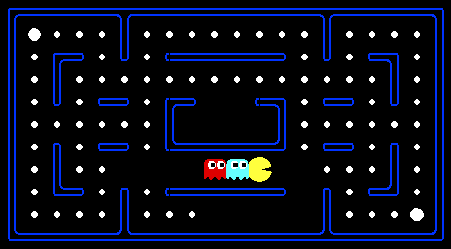
\includegraphics[width=12cm]{images/pacman_multi_agent} \par
		\vfill \par	\vfill
		\vspace{16mm}
		{\normalsize	سیدمحمدحسین هاشمی  4022363143 \par}
		
		\vspace{1cm}
		{\large دی ۱۴۰۲\par}
	\end{titlepage}
	\tableofcontents
	\newpage
	
	
	\section{توابع هیوریستیک \lr{(heuristic)}} \label{heuristic}
	
		{\normalsize از این توابع برای امتیاز دهی دقیق‌تر حالت ها استفاده می‌کنیم که هم حرکت‌های دقیق‌تری داشته باشیم و هم اینکه به لیل عمق محدود درخت بازی عامل در صورت عدم حضور عامل تاثیرگذار در امتیاز به دلیل بکسان بودن حرکت ها عمل \lr{Stop} را بصورت مداوم انتخاب می‌کند تا وقتی عامل تاثیر گذاری وارد محدوده بررسی عامل شود و در این صورت عامل بهترین بازی ممکن را انجام نمی‌دهد که برای هدایت عامل از این توابع استفاده می‌کنیم.}
		
		\subsection{\lr{heuristicFood}} \label{heuristicFood}
		
			\begin{center}
					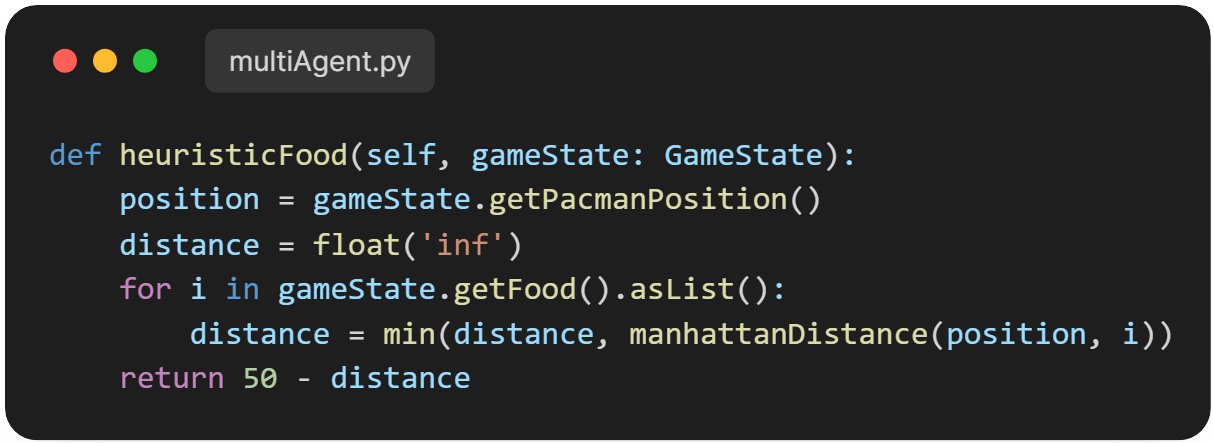
\includegraphics[width=12cm]{images/01}
			\end{center}
			
			{\normalsize این تابع بر اساس نزدیکی \lr{Pacman} به نزدیک ترین خانه غذا امتیاز می‌دهد.}
			
			
		\subsection{\lr{heuristicLastFood}}
		
			\begin{center}
				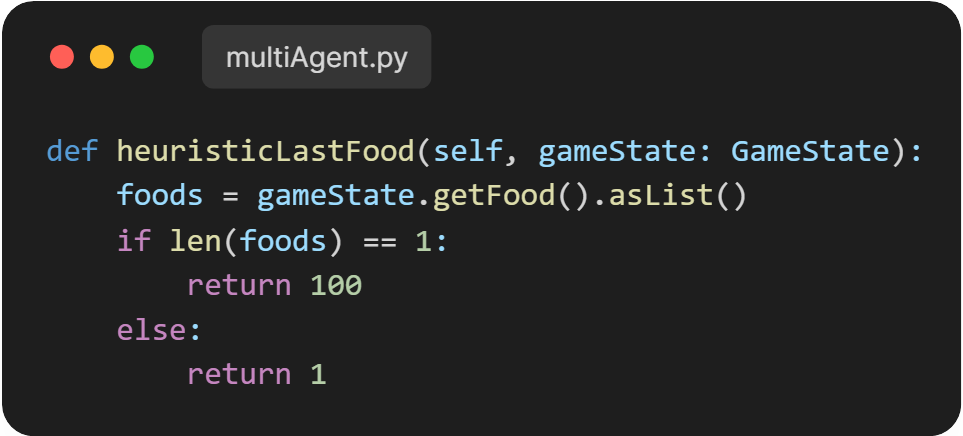
\includegraphics[width=12cm]{images/02}
			\end{center}
			
			{\normalsize این تابع در صورتی که تنها یک غذا باقی مانده باشد عدد \lr{100} و در غیر اینصورت عدد \lr{1} را برمیگرداند که از آن به عنوان ضریبی برای \ref{heuristicFood} استفاده می‌کنیم.}
	
	
		\subsection{\lr{heuristicGhost}}
		
			\begin{center}
				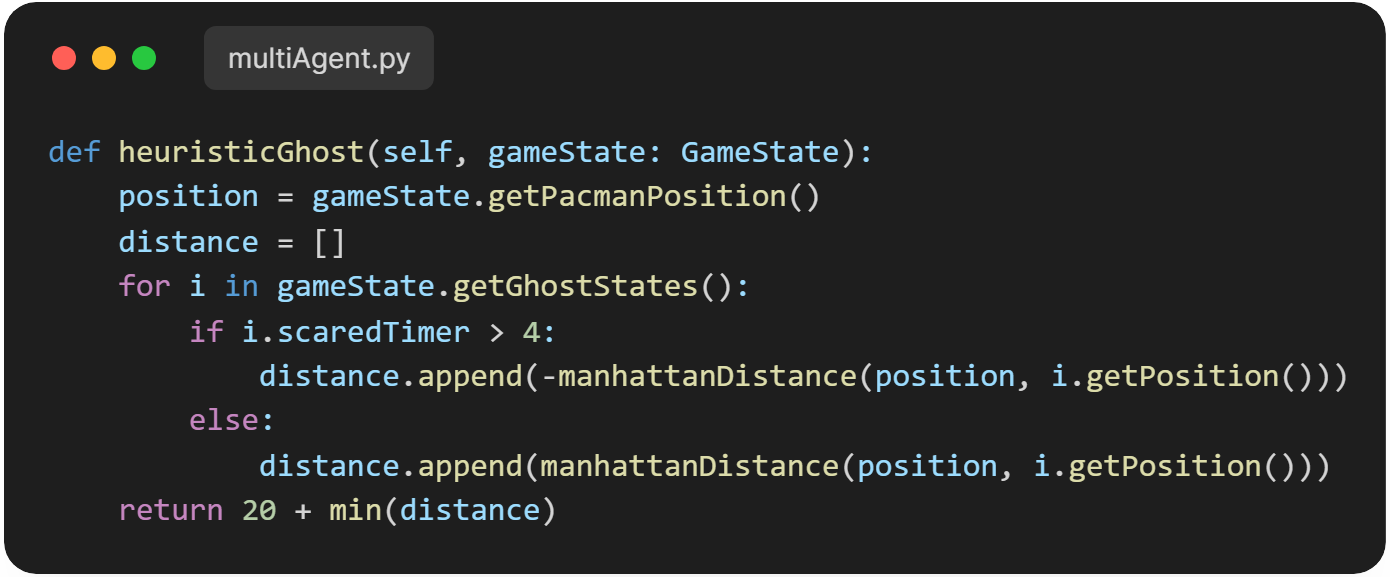
\includegraphics[width=12cm]{images/03}
			\end{center}
			
			{\normalsize این تابع بر اساس نزدیکی به روح‌های بازی امتیاز بندی می‌کند و دو حالت دارد:}
			
			\begin{itemize}
				\item {\small نزدیک بودن به روح ترسیده امتیاز بالاتری دارد.}
				
				\item {\small نزدیک بودن به روح در حالت معمول امتیاز کمتری دارد.}
			\end{itemize}
			
			
		\subsection{\lr{heuristicScaredGhost}}
		
			\begin{center}
				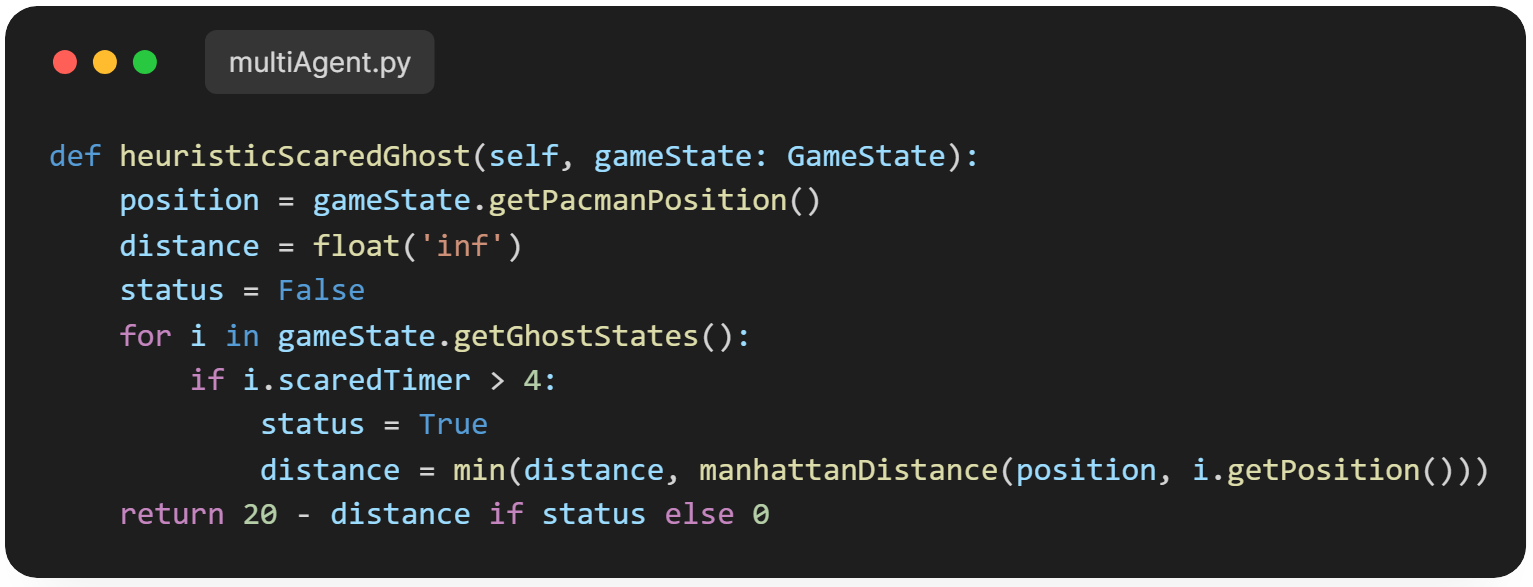
\includegraphics[width=12cm]{images/04}
			\end{center}
			
			{\normalsize این تابع برای نزدیکی به نزدیک ترین روح ترسیده امتیاز دهی می‌کند و در غیر اینصورت امتیاز \lr{0} را برمی‌گرداند.}
		
	
	\section{پردازش \lr{Minimax}}
	
		\subsection{\lr{Handler}} \label{Handler}
	
			\begin{center}
				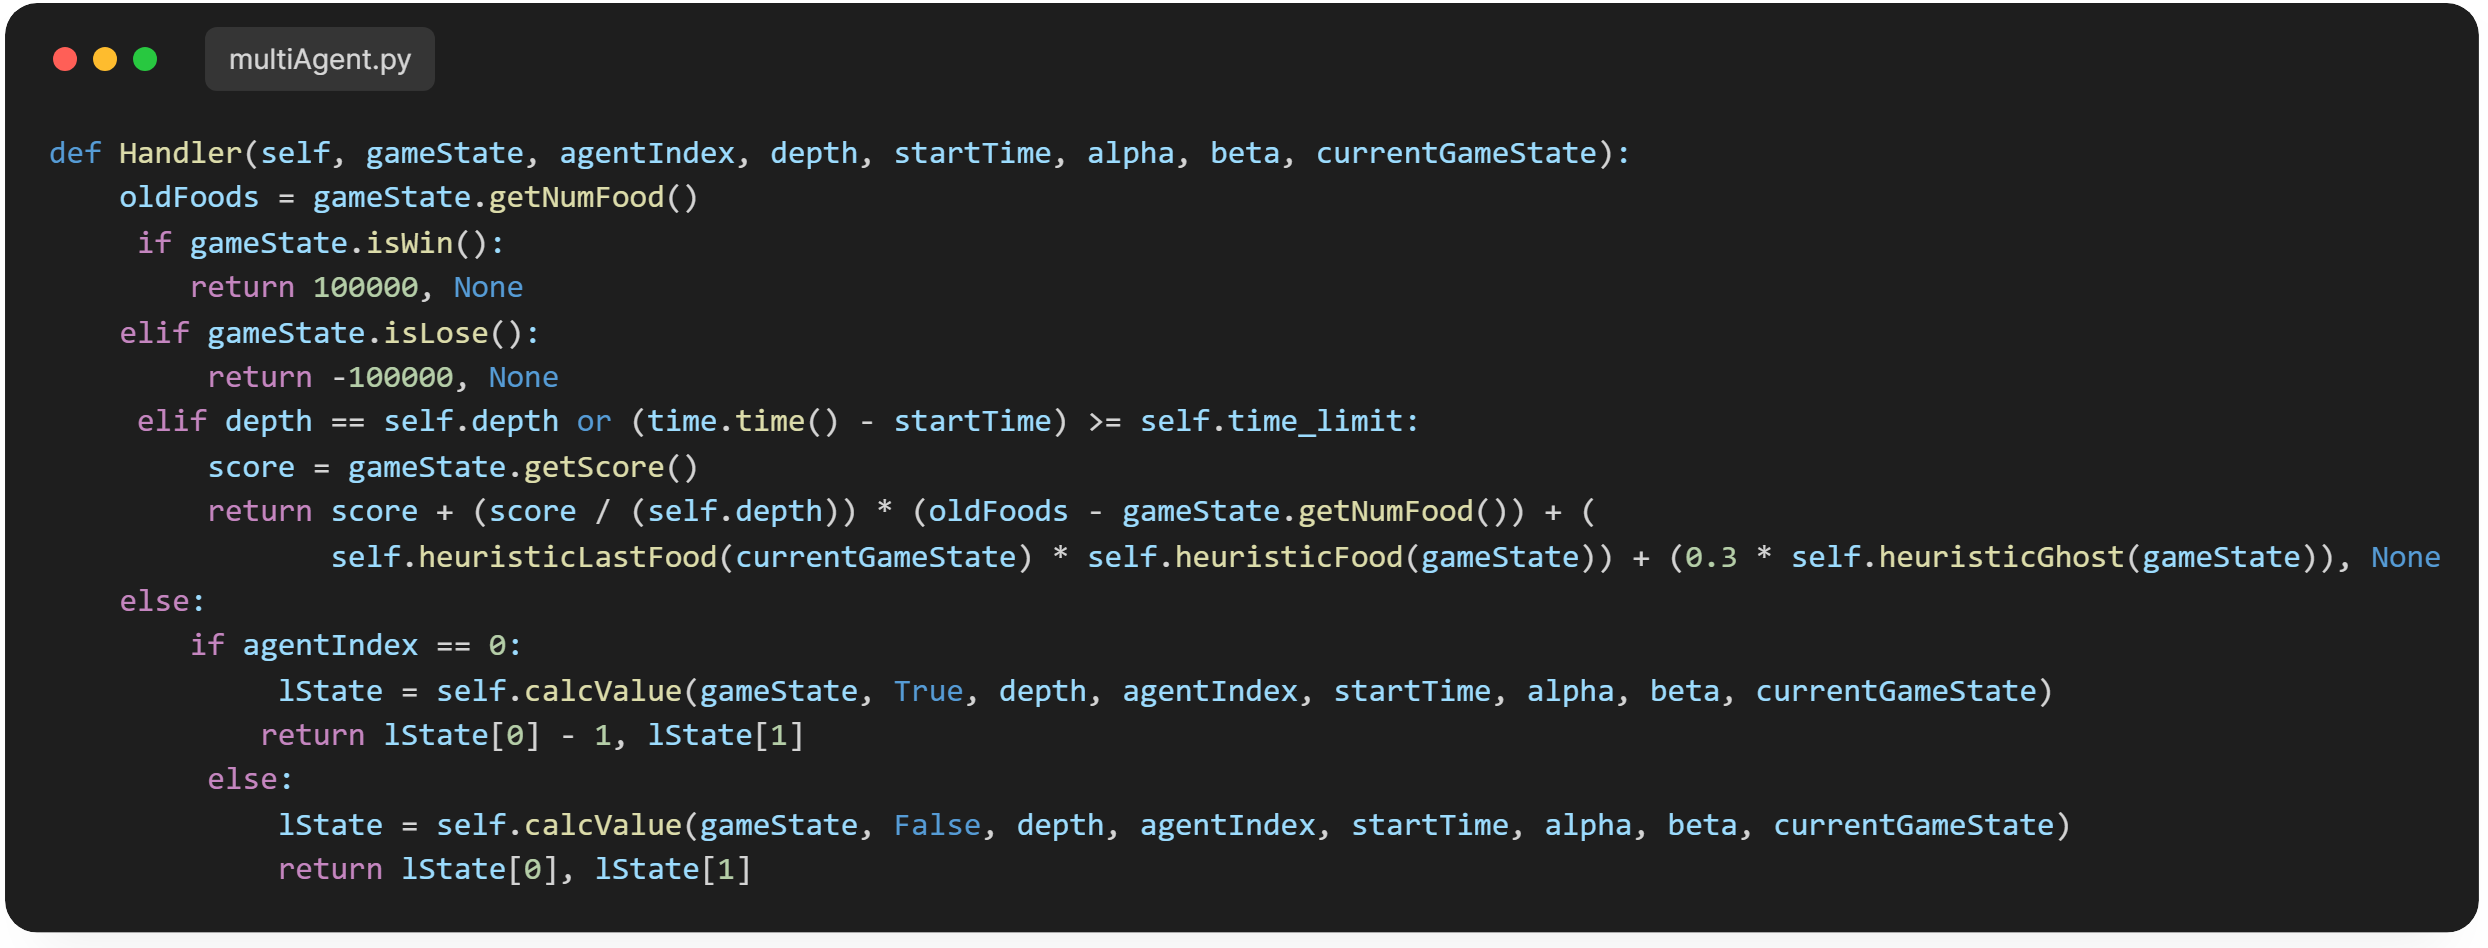
\includegraphics[width=12cm]{images/05}
			\end{center}
		
			{\normalsize این تابع بصورت بازگشتی اجرا شده و مانند درخت \lr{Minimax} حالت‌های ممکن را بررسی می‌کند و بهترین اکشن را با استفاده از بخش \ref{calcValue} محاسبه و برمی‌گرداند. همچنین در این تابع دو محدودیت زمان پردازش و عمق نیز قرار داده‌ایم. این درخت برای اخرین مقادیر ارزش ها را براساس حالت بازی و همچنین ارزش وضعیت‌ها و مقادیر بخش \ref{heuristic} تولید می‌کند.}
		
		
		\subsection{\lr{calcValue}} \label{calcValue}
		
			\begin{center}
				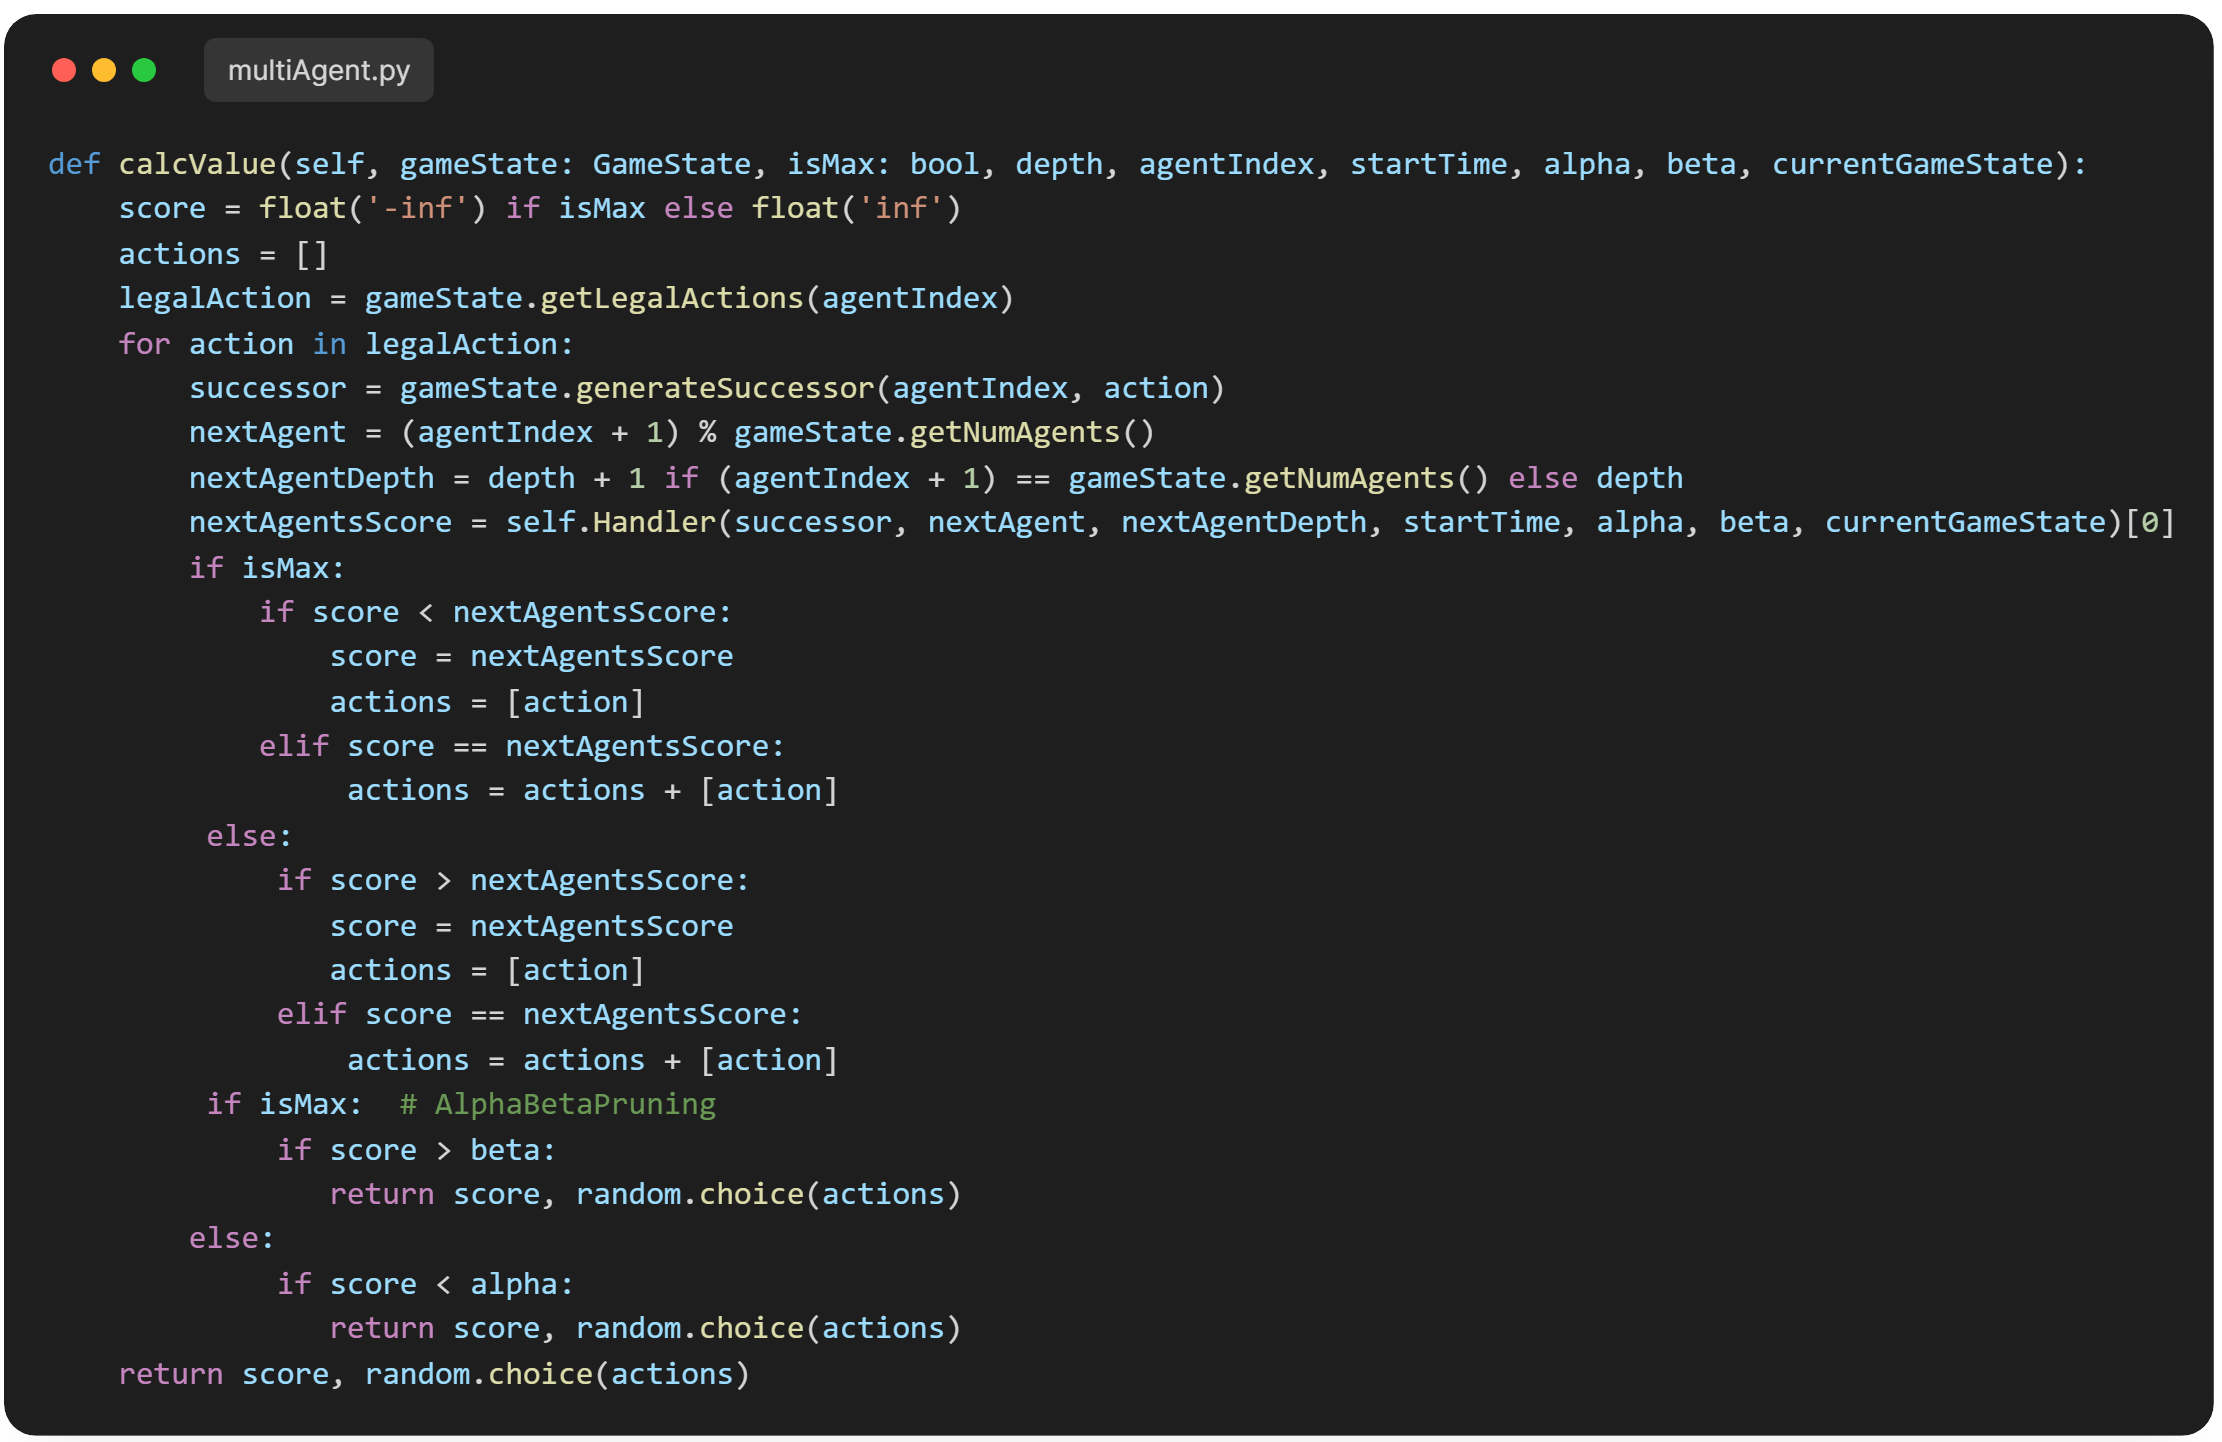
\includegraphics[width=12cm]{images/06}
			\end{center}
		
			{\normalsize این تابع همان بخش اجرایی برای پردازش درخت \lr{Minimax} است که توسط بخش \ref{Handler} فراخوانی می‌شود. در این تابع علاوه بر پردازش گفته شده حرص آلفابتا \lr{(AlphaBeta Pruning)} نیز انجام می‌شود.}
	
	
	\section{\lr{getAction}} \label{getAction}
	
		\begin{center}
			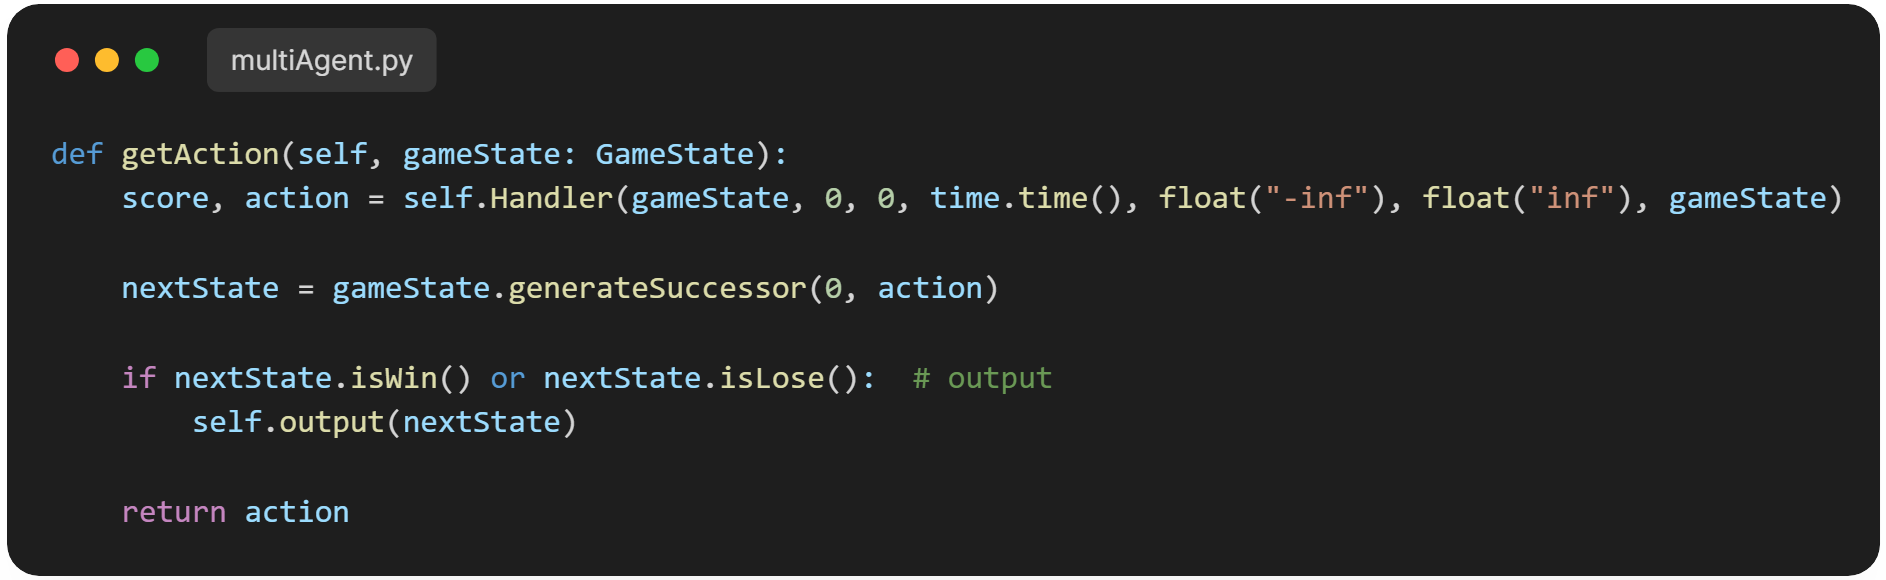
\includegraphics[width=12cm]{images/07}
		\end{center}
		
		{\normalsize این تابع وضعیت فعلی را به بخش \ref{Handler} داده و حرکتی فعلی \lr{Pacman} را دریافت و انرا برمی‌گرداند.}
		
		
	\section{\lr{output}}
	
		\begin{center}
			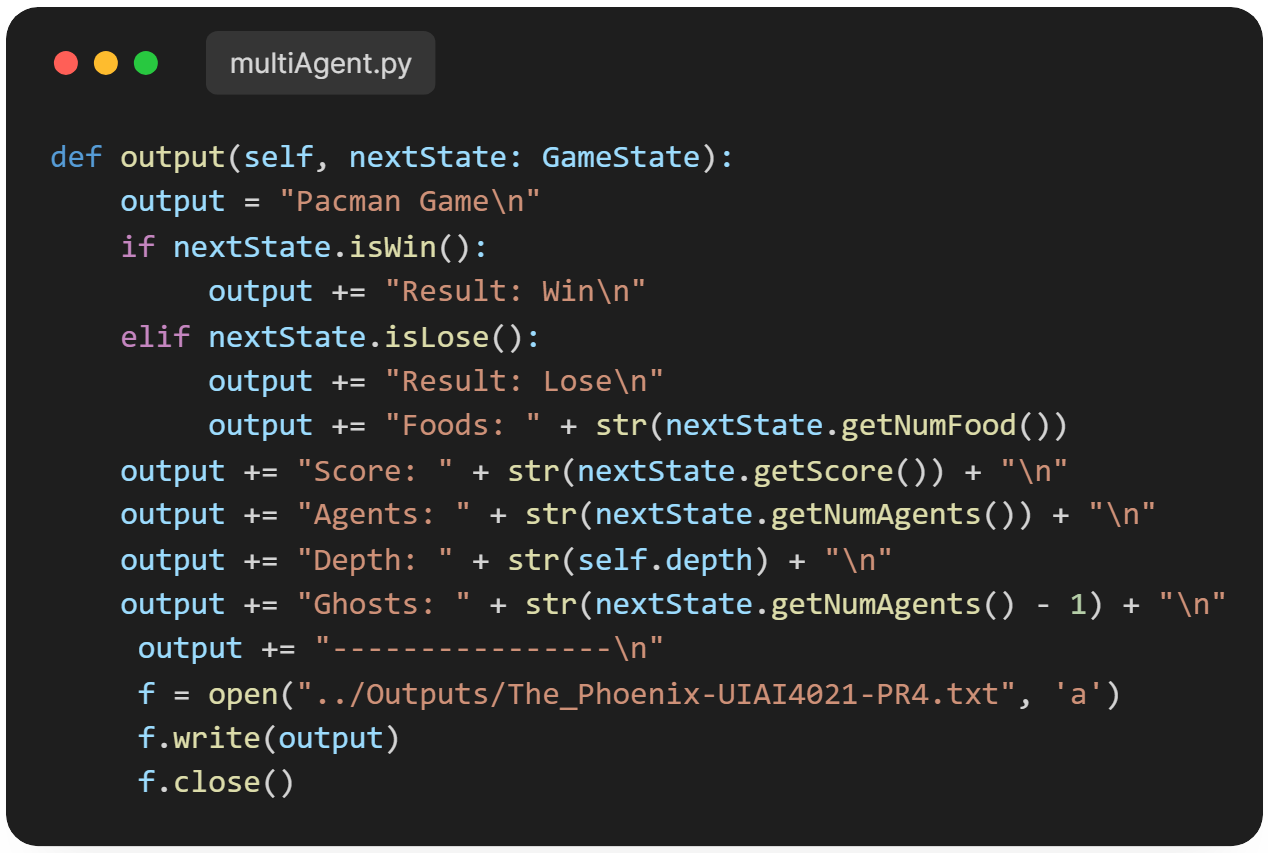
\includegraphics[width=12cm]{images/08}
		\end{center}
	
		{\normalsize در نهایت این تابع خروجی به فرم زیر تولید و ذخیره می‌کند.}
		
		\begin{center}
			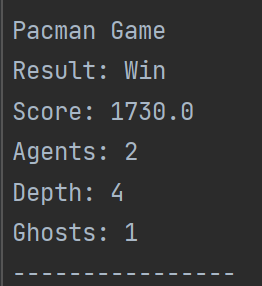
\includegraphics[width=5cm]{images/09}
		\end{center}
	
	
	
\end{document}